\documentclass{uai2025} % for initial submission
%\documentclass[accepted]{uai2025} % after acceptance, for a revised version; 
% also before submission to see how the non-anonymous paper would look like 
                        
%% There is a class option to choose the math font
% \documentclass[mathfont=ptmx]{uai2025} % ptmx math instead of Computer
                                         % Modern (has noticeable issues)
% \documentclass[mathfont=newtx]{uai2025} % newtx fonts (improves upon
                                          % ptmx; less tested, no support)
% NOTE: Only keep *one* line above as appropriate, as it will be replaced
%       automatically for papers to be published. Do not make any other
%       change above this note for an accepted version.

%% Choose your variant of English; be consistent
\usepackage[american]{babel}
% \usepackage[british]{babel}

%% Some suggested packages, as needed:
\usepackage{natbib} % has a nice set of citation styles and commands
    \bibliographystyle{plainnat}
    \renewcommand{\bibsection}{\subsubsection*{References}}
\usepackage{mathtools} % amsmath with fixes and additions
% \usepackage{siunitx} % for proper typesetting of numbers and units
\usepackage{booktabs} % commands to create good-looking tables
\usepackage{tikz} % nice language for creating drawings and diagrams

\usepackage{amsmath}
\usepackage{amssymb}
\usepackage{amsthm}
\usepackage{todonotes}
\usepackage{bm}
\usepackage{subcaption}
\usepackage[linesnumbered, ruled]{algorithm2e}

\def\ci{\perp\!\!\!\!\!\perp}

\newtheorem{definition}{Definition}
\newtheorem{proposition}{Proposition}
\newtheorem{theorem}{Theorem}

\title{Expert-In-The-Loop Causal Discovery: Iterative Model Refinement Using Expert Knowledge}

% The standard author block has changed for UAI 2025 to provide
% more space for long author lists and allow for complex affiliations
%
% All author information is authomatically removed by the class for the
% anonymous submission version of your paper, so you can already add your
% information below.
%
% Add authors
\author[1]{\href{mailto:<ankur.ankan@ru.nl>?Subject=Your UAI 2025 paper}{Ankur~Ankan}{}}
\author[1]{Johannes~Textor}

% Add affiliations after the authors
\affil[1]{%
    Institute for Computing and Information Sciences\\
    Radboud University\\
    Nijmegen, The Netherlands
}
\begin{document}

\maketitle

\begin{abstract}

	Causal discovery has received significant attention in the Directed
	Acyclic Graphs (DAGs) literature, leading to the development of
	numerous automated algorithms for learning DAGs from data. However,
	their adoption in applied domains remain limited, as researchers often
	prefer to construct DAGs manually based on domain knowledge. This
	preference arises due to several practical challenges with automated
	algorithms, such as their tendency to make obvious errors and output
	Markov Equivalence Classes (MECs) rather than a DAG. To assist
	researchers in constructing DAGs manually, we propose an iterative DAG
	construction approach that combines domain knowledge with data-driven
	insights. Our method leverages Conditional Independence (CI) testing to
	iteratively identify variable pairs where an edge is either missing or
	superfluous. Based on this information, we can choose to add missing
	edges with appropriate orientation based on domain knowledge or remove
	unnecessary ones. We also give a method to rank potential new edges
	based on their impact on the overall model fit. Empirical results show
	that this iterative approach achieves performance comparable to
	automated algorithms if the orientation of new edges is correctly
	determined in at least one out of two cases. Additionally, we show
	that, in the absence of an expert, a Large Language Model (LLM) can be
	used to determine edge orientations. We provide an implementation of
	our approach as both a webtool: <redacted for review> and a Python
	package <redacted for review>.

\end{abstract}

\section{Introduction}
Understanding cause-and-effect relationships between variables is a fundamental
objective in many scientific fields. These relationships reveal the mechanisms
behind observed phenomena and guide effective interventions or policy
decisions. Causal discovery methods aim to discover such relationships
among random variables using observational data. 

% Approaches to causal discovery
% have been developed within both the Directed Acyclic Graphs (DAGs) and
% Structural Equation Models (SEMs) frameworks, each adapting a different
% approach.

In the DAG literature, the primary focus has been on developing automated
algorithms to learn causal structures from datasets. These efforts have led to
numerous causal discovery algorithms, such as constraint-based methods like PC
algorithm \citep{Spirtes2001} and Fast Causal Inference \citep{Spirtes2000}),
score-based methods such as Hill-Climb Search and Greedy Equivalence Search
\citep{Chickering2002}, and continuous optimization-based methods like NO TEARS
\citep{Zheng2018} and DAGMA \citep{Bello2022}. Despite significant progress in
automated causal discovery, their adoption in applied research has been
limited. Researchers often prefer to manually construct DAGs based on their
domain expertise \citep{Tennant2020, Petersen2021}. We attribute this
preference to several challenges with existing causal discovery algorithms in
practical settings:

\begin{enumerate}
	\item \textbf{Lack of Trust:} While most algorithms are asymptotically
		consistent, their behavior on finite samples is not well
		understood. Their output can vary significantly depending on
		the choice of algorithm and hyperparameters, making it
		difficult to assess reliability. Additionally, the absence of
		robust performance evaluation methods for any given dataset
		further reduce the confidence in their outputs. 
	\item \textbf{Outputs Markov Equivalence Class (MEC):} As multiple
		DAGs can be faithful to a given observational dataset, automated 
		algorithms can only recover the MECs. These MECs can contain a
		combination of directed and undirected edges. However, most
		methods for downstream tasks, such as identification or causal
		effect estimation, assume knowledge of a fully oriented DAG. 
\end{enumerate}

Figure~\ref{fig:intro} highlights some of these issues. Constructing DAG
manually, on the other hand, can also be error prone as it can be difficult to
distinguish various scenarios such as direct or indirect effects, mediation,
and so on. This makes it important to test the consistency of our DAG against
our dataset. One of the methods for testing this is to check whether the
implied CIs of the DAG hold in the dataset or not \citep{Ankan2021}. Each pair
of variables with a missing edge between them in the DAG implies a CI
statement, we can use a statistical test to check whether the statement holds
in our dataset or not. If we find any violations we can also modify our DAG
based on this and utilizing our domain knowledge to find a suitable orientation
for the edge between the pair of variables.

% While DAG-based methods focus on
% automated discovery, SEM-based methods emphasize expert driven model
% specification. This includes tools to assist researchers in manually
% constructing models, enabling them to incorporate their domain knowledge in the
% model building process. Researchers typically begin with an initial model based
% on their domain knowledge and then use these tools to guide modifications that
% improve the model's fit to data. This process is commonly known as
% Specification Search \citep{Long1983} and uses method such as modification
% indices, and Wald-based tests \citep{Marcoulides2018}. 

In this paper we present a method that utilizes this idea of CI testing to
assist researchers during the DAG construction instead of testing the final
model. We propose an iterative model construction method that combines domain
knowledge with data-driven insights. Our approach utilizes conditional
independence testing to identify pair of variables in the DAG that are missing
an edge or have a superfluous edge. Based on this information, in each
iteration we present one such pair of variables to an expert who then decides
the orientation of the edge between the variables based on their domain
knowledge. The method also iteratively prunes all superfluous edges in each
iteration. As a result this approach guides the expert in constructing their
model while ensuring that the model is consistent with the data.

As at any iteration, multiple changes to the DAG are possible. We also give a
way to rank potential new edges additions to the DAG using effect size measures
for CI tests.

% When manually constructing models, it is important to test whether the
% resulting DAG accurately represents the dataset. Based on this evaluation and
% domain knowledge, we can make further modification to the model. One common
% approach for assessing DAGs is to check whether the Conditional Independences
% (CIs) implied by the DAG hold in the data \citep{Ankan2021}. If we find
% violations to these CIs, we can use our domain knowledge to make appropriate
% modifications to the DAG. However, this CI testing approach has a few
% limitations:
% 
% \begin{enumerate}
% \item As CIs are only implied by missing edges in the model, this approach does 
% 	not test whether the existing edges are correct.
% \item Determining whether a CI holds in data is based on a p-value threshold. This can 
% 	be unreliable, for example, we get a significant p-value for even very weak 
% 	relationship if the sample size is high.
% \item The number of implied CIs can be large making it difficult to manually
% 	check all of them. For example, a moderately sized alarm network
% 	\citep{Beinlich1989} with $ 37 $ nodes, implies $ 287 $ CIs.
% \end{enumerate}
% 
% To tackle these limitations, we draw inspiration from modification indices in
% specification search. Modification indices provide ranking for potential model
% modification based on their impact on the model's fit, allowing us to
% prioritize most meaningful modifications.  Similarly, we propose a method for
% ranking CI test violations to help us focus on the most critical
% inconsistencies in the model. To determine this ranking we utilize a measure of
% conditional association between variables in combination with p-values from the
% CI test. This approach addresses all three of the issues outlined above. The
% measure of association allows us to evaluate the validity of existing edges. It
% reduces our reliance on p-values alone for deciding whether the CI test holds.
% The ranking helps us prioritize the most critical violations, making it feasible 
% to focus on the areas that most improve the model's fit.

\begin{figure}[t!]
    \begin{subfigure}{0.5 \textwidth}
	\centering
    	\includegraphics[page=1]{figures_v2.pdf}
    	\caption{}
    \end{subfigure}
    \begin{subfigure}{0.5\textwidth}
	\centering
    	\includegraphics[page=2]{figures_v2.pdf}
    	\caption{}
    \end{subfigure}
    \begin{subfigure}{0.5\textwidth}
	\centering
    	\includegraphics[page=3]{figures_v2.pdf}
    	\caption{}
    \end{subfigure}

    \caption{A comparison of Markov Equivalence Class (MEC) learned using Adult
	     Income Dataset \citep{Becker1996} using different causal discovery
	     algorithms and sample sizes. Edge colour represents the sample size
	     used: red ($N=400$), and blue ($N=800$). (a) PC algorithm with a
	     mutual information based CI test, (b) PC algorithm with a
    	     residualization based test \citep{Ankan2023}, (c) Hill Climb Search with
	     Bayesian Information Criterion (BIC) score. The learned model structure varies
             significantly in each case.}
    \label{fig:intro}
\end{figure}


Our main contributions in this paper are as follows:

\begin{enumerate}
%     \item We propose a novel measure of conditional association for mixed data
% 	    based on canonical correlations
% 	    (Section~\ref{sec:mixed_association}). This measure generalizes
% 	    several commonly used special case measures of association to mixed
% 	    data.
    \item We develop an iterative method based on CI testing to assist researchers in 
	    constructing DAGs using their domain knowledge (Section~\ref{sec:modification}).
    \item We develop a ranking method to prioritize potential modifications in the DAG that 
    	    can help in improving the model's fit quickly (Section~\ref{sec:ranking}).
    \item We provide a web-based interactive tool and a Python package to allow 
	    researchers to easily apply this method to their datasets (Section~\ref{sec:web}).
    \item Lastly, we compare the manual DAG construction method with automated
	    causal discovery algorithms (Section~\ref{sec:empirical}).
\end{enumerate}

% The rest of the paper is structured as follows. In
% Section~\ref{sec:background}, we give a background on the commonly used
% measures of association for various data types. In
% Section~\ref{sec:mixed_association}, we present our generalized measure of
% conditional association for mixed data. Section~\ref{sec:modification} provides
% details on the procedure for using the measure of association for constructing
% DAGs. Section~\ref{sec:web} presents our web-browser based tool and lastly in
% Section~\ref{sec:empirical}, we show some empirical results to compare this
% manual DAG construction approach to automated algorithms.

\section{Background and Related Work}
\label{sec:background}
\todo[inline]{Need to rewrite this}
We denote random variables with uppercase letters $ X $, and a set of random
variables as $ \bm{X} = \{X_1, \cdots, X_k\} $ with $ \rvert \bm{X} \rvert = k
$. A sample from the random variable $ X $ is denoted as $ x $ and from a set
of random variables $ \bm{X} $ is denoted as $ \bm{x} $. In this paper, we
consider random variables in the mixed data setting where each of the random
variables can be either of continuous, categorical, or ordinal unless
specified. We write the expectation of a variable $ X $ as $ \mathbb{E}[X] $,
conditional expectations as $ \mathbb{E}[X | \bm{Z}] $. We denote a graph $ G =
(V, E) $ which nodes $ V$ and edges $ E $. In this paper we focus on all
observed variables, and linear measure of association. 
where $ \mathrm{cov}(X, Y) $ is the covariance between $ X $ and $ Y $, $ \mathrm{corr}(X, Y) $ is the correlation between $ X $ and $ Y $, and $
\sigma_X $ and $ \sigma_Y $ are the standard deviations of $ X $ and $ Y $
respectively.  Covariance matrix using $ \Sigma $ and the entry corresponding to
covariance between $ X $ and $ Y $ in the matrix using $ \Sigma_{XY} $.

\subsection{Integrating domain knowledge in causal discovery}
Multiple ways to integrate, originally using forbidden and required edges. Or
temporal algorithms by specifying causal tiers.

\subsection{Measures of Conditional Association}
Our approach for ranking CI tests is based on a measure of conditional
association -- also known as partial association -- between variables.
Specifically, we are interested in quantifying the association between
variables $ X $ and $ Y $ when conditioned on a set of variables $ \bm{Z} $
(which may be empty, i.e., $ \bm{Z} = \emptyset $). Various measures of
conditional association have been used for this purpose depending on the type
of $ X $, $ Y $, and $ \bm{Z} $. These measures are often based on the effect
size of the CI test $ X \ci Y \rvert \bm{Z} $. In this section, we give an
overview of some of the commonly used measures for different data types.

\paragraph{Both $ X $ and $ Y $ are continuous: }
When both $ X $ and $ Y $ are continuous, Pearson's correlation coefficient is
typically used. When $ \bm{Z} = \emptyset $, the correlation
coefficient is defined as:

\begin{equation}
	r_{X, Y} = \frac{\mathrm{cov}(X, Y)}{\sigma_X \sigma_Y}
\end{equation}

When $ \bm{Z} \neq \emptyset $, partial correlation coefficient can be used.
This is estimated by fitting two regression models $ E_X: X \sim \bm{Z} $ and $
E_Y: Y \sim \bm{Z} $, calculating the residuals $ R_X = X - E_X(\bm{Z}) $ and $
R_Y = Y - E_Y(\bm{Y}) $, and then computing the correlation between the
residuals:

\begin{equation}
	r_{X, Y; \bm{Z}} = r_{R_X, R_Y}
\end{equation}

\paragraph{All $ X $, $ Y $, and $ \bm{Z} $ are discrete: }

When all variables are discrete, Cram\'er's V can used as a measure of
association. When $ \bm{Z} = \emptyset $, Cram\'er's V is derived from the 
chi-squared test statistic:

\begin{equation}
	\mathbf{V}_{X, Y} = \sqrt{\frac{\chi^2 / n}{\mathrm{min}(k-1, r-1)}}
\end{equation}

where $ \chi^2 $ is the chi-squared test statistic for $ X $ and $ Y $, $ n $
is the sample size, and $ k $ and $ r $ are the number of categories in $ X $
and $ Y $ respectively. When $ \bm{Z} \neq \emptyset $, we start by splitting
the dataset by each unique combination of $ \bm{Z} $ into subsets,  $ \bm{Z} $,
$ D = \{ D_{\bm{Z} = \bm{Z}_1}, D_{\bm{Z} = \bm{Z}_2}, \cdots, D_{\bm{Z} =
\bm{Z}_k} \} $. Then we compute the Cram\'er's V for each of these smaller datasets
and combine them as follows:

\begin{equation}
	\mathbf{V}_{X, Y; \bm{Z}} = \sum_{i=1}^{k} \left[ \mathbf{V}_{X, Y} \right]_{D_{\bm{Z} = \bm{Z}_i}} 
\end{equation}

\paragraph{$ X $ is ordinal, and $ Y $ and $ Z $  are continuous or ordinal: }

Polyserial (when one is ordinal and the other is continuous) and Polychoric
(when both are ordinal) correlation have been used to estimate the covariance
matrix between them \citep{Poon1987}. Both methods make the assumption that the
observed ordinal variable is a result of thresholding a latent normally
distributed continuous variable. Under this assumption, the methods then try to
estimate the covariance matrix while maximizing the likelihood of the dataset.
Using the estimated covariance matrix, $ \Sigma $ we can the compute Pearson's
correlation coefficient. When $ \bm{Z} = \emptyset $,

\begin{equation}
	r_{X, Y} = \frac{\Sigma_{XY}}{\sqrt{\Sigma_{XX} \Sigma_{YY}}}
\end{equation}

When $ \bm{Z} \neq \emptyset $, 

\begin{equation}
	r_{X, Y; \bm{Z}} = - \frac{\Sigma^{-1}_{XY}}{\sqrt{\Sigma^{-1}_{XX} \Sigma^{-1}_{YY}}}
\end{equation}


\section{DAG Structure Learning using Ancestral Oracles}
\label{sec:modification}

Our approach to causal structure learning combines domain knowledge with data-driven
insights in a manner that is based on the following considerations: 
(1) A domain experts is possibly good at determining causal directions between variables if 
there is a clear causal direction between them. (2) A domain expert may be less good
at identifying cases where there is no causal relationship between the variables,
since \emph{potential} causal relationships can often be argued for anyway.
(3) Many domain experts could struggle to distinguish direct from indirect 
effects, since the presence of a direct effect between two variables
of interest depends on all other variables present in the graph. 

We therefore consider the following two models of a domain experts: Given two variables
$ X $ and $ Y $ that are part of an unknown causal DAG $G$, an \emph{strong ancestral oracle} 
$\mathcal{A}_G$ is defined as:
$$\mathcal{A}_G(X,Y)=\begin{cases}
 X \to Y & \textrm{if } X \in \textrm{An}_G(Y) \\
 X \gets Y & \textrm{if } Y \in \textrm{An}_G(X) \\
 \textrm{None} & \textrm{otherwise} \\
\end{cases}$$

whereas a \emph{weak ancestral oracle} is defined as:
$$
\mathcal{A}_G(X,Y)=\begin{cases}
 X \to Y & \textrm{if } X \in \textrm{An}_G(Y) \\
 X \gets Y & \textrm{if } Y \in \textrm{An}_G(X) \\
 \textrm{rand}(X \gets Y, X \to Y) & \textrm{otherwise} \\
\end{cases}
$$

That is, our ancestral oracles only provide information on the direction of cause-effect
relationships, and do not distinguish between direct and indirect effects. 
The weak ancestral oracle is even unable to detect cases where there is no cause-effect
relationship between two variables. Using such oracles for DAG construction therefore 
inherently risks that superfluous edges are created. In our approach, such superfluous edges
will be detected and removed by utilizing the data. 

To model how our learning procedure interacts with the data, we assume that we
additionally have access to a second oracle $\mathcal{D}_G$ than can answer d-separation
queries with respect to the unknown target graph:
$\mathcal{D}_G(X,Y,\mathbf{Z})=1$ iff $X$ and $Y$ are $d$-separated by $\mathbf{Z}$ in 
$G$. These are the standard oracles considered in constraint-based structure learning
algorithms, such as the PC algorithm \cite{Spirtes2001}. 

Based on these two oracles, we now define two core procedures that we will use to 
iteratively change a current DAG structure. The procedure 
\textsc{Expand} (Algorithm~\ref{algo:expand}) uses conditional independence
information to search for missing edges in the graph and then uses domain
knowledge to orient them. The procedure \textsc{Prune} (Algorithm~\ref{algo:prune}) uses
conditional independence information to remove superfluous edges from the
graph.

\begin{algorithm}[h]
\DontPrintSemicolon
\SetAlgoLined
\SetKwFunction{Expand}{Expand}
\SetKw{KwGoTo}{go to}
\SetKwProg{Fn}{Function}{:}{}
\Fn{{\sc Expand}($V,E,\mathcal{D}_G,\mathcal{A}_G$,$B$,$k$)}{
    let $L \gets \{\}$\;
    \ForEach{$X, Y$ where $X \to Y \notin E$ and $Y \to X \notin E$ and 
	$\{X,Y\} \notin B$}{
        let $\mathbf{Z}$ be a set that $d$-separates $X$ and $Y$ in $(V,E)$\;
        \If{$\mathcal{D}_G(X, Y, \mathbf{Z}) = 0$}{
	    $e \gets \mathcal{A}_G(X, Y)$ \;
	    \uIf{ $(V,E \cup L \cup e)$ is acyclic }{
            	$L \gets L \cup  \{ e \} $\;
	    } \Else {
            	$L \gets L \cup  \{ \textrm{reverse}(e) \} $\;
	    }
        }
	\If{$|L|\geq k$}{\KwGoTo 12\;}
    }
    add all edges in $L$ to $E$\;
    \Return{$(V,E)$}\;
}
\caption{Adding edges based on data and domain knowledge.}
\label{algo:expand}
\end{algorithm}

The function $\textsc{Expand}$ takes an initial list of edges and searches for 
any vertex pairs that are not connected but where the d-separation oracle 
indicates  that there is still a residual association not explained by the other variables.
An optional parameter $B$, the empty set by default, allows to specify a ``black list''
of vertex pairs that must not be connected, and another optional parameter $k$
specifies the maximum amount of edges to be added by this procedure.

Let $G^+$ denote the transitive closure of $G$, that is, the graph in which 
there is a direct edge $X \to Y$ whenever $X \in \textrm{An}_G(Y)$. The transitive
closure is related to the result of $\textsc{Expand}$ by the following two 
easily proved facts.

\begin{proposition}
For a conditional independence oracle
 $\mathcal{D}_G$ and a strong ancestral oracle $\mathcal{A}_G$, 
$\textsc{Expand}(V,\emptyset,\mathcal{D}_G,\mathcal{A}_G, \emptyset, \infty)=G^+$.
\label{prop:strongexpand}
\end{proposition}

\begin{proof}
Since we start from an empty graph, every pair of vertices $X, Y$ where
 $X \in \textrm{An}_G(Y)$ is d-separated by the empty set and is
 connected by the edge $X \to Y$. No other edges are added. Therefore, 
the result is $G^+$. 
\end{proof}

\begin{proposition}
For a conditional independence oracle
 $\mathcal{D}_G$ and a weak ancestral oracle $\mathcal{A}_G$, 
$\textsc{Expand}(V,\emptyset,\mathcal{D}_G,\mathcal{A}_G, \emptyset, \infty)
\supseteq G^+$.
\label{prop:weakexpand}
\end{proposition}

\begin{proof}
Every pair of vertices $X, Y$ that are $d$-connected in $G$ are now connected by an edge 
during $\textsc{Expand}$. For $X \in \textrm{An}_G(Y)$, the edge is 
$X \to Y$ just like when using a strong ancestral oracle; since only correctly oriented
edges are added between ancestor-descendant pairs, such additions never create cycles.
For $X, Y$ that are only $d$-connected throug common ancestors, an arbitrary 
edge is added in a manner that preserves acyclicity. The result is a supergraph
of $G^+$.
\end{proof}


\begin{algorithm}[h]
\DontPrintSemicolon
\SetAlgoLined

\SetKwProg{Fn}{Function}{:}{}
\Fn{{\sc Prune}($V$,$E$,$\mathcal{D}_G$)}{
    let $L \gets \{\}$\;
    \ForEach{$X \to Y \in E$}{
        remove $X \to Y$ from $E$\;
        let $\mathbf{Z}$ be a set that $d$-separates $X$ and $Y$ in $(V,E)$\;
        \If{$\mathcal{D}_G(X, Y, \mathbf{Z}) = 1$}{
            $L \gets L \cup  \{X \to Y\}$ \;
        }
    }
    remove all edges in $L$ from $G$\;
    \Return{$(V,E)$}\;
}
\caption{Pruning superfluous edges}
\label{algo:prune}
\end{algorithm}

Unlike our ancestral oracles, the pruning operation is quite effective at distinguishing
direct and indirect effects, as shown by the following result.

\begin{proposition}
Consider two DAGs $G=(V,E)$ and $G'=(V,E')$ where $E \subseteq E'$. 
Then $\textsc{Prune}(G',\mathcal{D}_G)=G$.
\label{prop:prune}
\end{proposition}

\begin{proof}
For an edge $X \to Y$ in the skeleton of $G$, $\mathcal{D}_G(X, Y, \mathbf{Z}) = 0$ regardless 
of $\mathbf{Z}$, so all edges in the skeleton are retained after {\sc Prune}. Conversely, if 
 $X \to Y$ is not in the skeleton of $G$, let $\mathbf{Z}$ be the $d$-separating set chosen 
in line~5 of {\sc Prune} (there is at least one such $\mathbf{Z}$, the union of the parents of 
$X$ and $Y$). Since  $\mathbf{Z}$ $d$-separates all paths from $X$ to $Y$ in $G'$, it does the same 
in $G$ which contains a subset of these paths. Therefore, all edges not in the skeleton of $G$ are 
removed.
\end{proof}

By combining Propositions~\ref{prop:strongexpand}, \ref{prop:weakexpand} and 
\ref{prop:prune}, we immediately obtain the following:

\begin{theorem}
Given a d-separation oracle $\mathcal{D}_G$ and a strong or weak 
ancestral oracle $\mathcal{A}_G$, 
$\textsc{Prune}(\textsc{Expand}((V,\emptyset),\mathcal{D}_G,\mathcal{A}_G,\emptyset,\infty),\mathcal{D}_G)=G.$
\end{theorem}

Since we require expert knowledge only in the $\textsc{Expand}$ operation, we may try
to be more economical by asking fewer questions at a time and interleaving expansion and
pruning steps. This leads us to the following, more incremental DAG construction algorithm.

\begin{algorithm}[h]
\DontPrintSemicolon
\SetAlgoLined
\SetKwProg{Fn}{Function}{:}{}

\Fn{{\sc ExpertInLoop}($V,\mathcal{D}_G,\mathcal{A}_G$)}{
$E_p \gets \emptyset$ \tcc{Current edges} 
$B \gets \emptyset$ \tcc{Edges that were pruned} 
\Repeat{ $E=E_p$ }{
	$E \gets E_p$ \;
	$(V,E) \gets \textsc{Expand}(V,E,\mathcal{D}_G,\mathcal{A}_G,B,1)$ \;
	$(V,E_p) \gets \textsc{Prune}(V,E,\mathcal{D}_G)$ \;
	$B \gets B \cup \{ E_p \setminus E \} $
}
\Return{(V,E)}
}

\caption{Iterative structure learning with expert in the loop}
\label{algo:expert}
\end{algorithm} 

\begin{theorem}
Let $G=(V,^*E)$ be a DAG, $\mathcal{D}_G$ a d-separation oracle for $G$, and 
$\mathcal{A}_G$ a strong or weak ancestral oracle for $G$. Then 
$\textsc{ExpertInLoop}(V,\mathcal{D}_G,\mathcal{A}_G)=G$.
\end{theorem}

\begin{proof}
The loop in Algorithm~\ref{algo:expert} terminates if and only if $E=E^*$. If the loop does not 
terminate, a new edge has been added in line 6, and/or one or more edges were pruned in line 7; the pruned 
edges never include the edge added in line 6 in the same iteration.
Every edge can be added at 
most once and pruned at most once. Therefore, the algorithm always terminates
after at most $|V|(|V|-1)+1$ iterations of the loop. For every edge $e=X\to Y $ in the skeleton of $G$, $\mathcal{D}_G(X,Y,\mathbf{Z})=0$ irrespective of $\mathbf{Z}$, and $e$ must be added to $E$ in some iteration, and can never be pruned afterwards. Therefore, after some iteration, $(V,E)$ must be a supergraph of $G$ after executing line 6, and this will be pruned to the real graph $G$ in line 7 (Proposition~\ref{prop:prune}). In the next iteration, no further changes are made, and the loop terminates.
\end{proof} 


\begin{figure}[t!]
	\begin{subfigure}{0.125 \textwidth}
		\centering
		\includegraphics[page=1]{example.pdf}
		\caption{True DAG}
	\end{subfigure}%
	\begin{subfigure}{0.125 \textwidth}
		\centering
		\includegraphics[page=2]{example.pdf}
		\caption{No edges.}
	\end{subfigure}%
	\begin{subfigure}{0.125 \textwidth}
		\centering
		\includegraphics[page=3]{example.pdf}
		\caption{$ X_1 \rightarrow X_4 $}
	\end{subfigure}%
	\begin{subfigure}{0.125 \textwidth}
		\centering
		\includegraphics[page=4]{example.pdf}
		\caption{$ X_1 \rightarrow X_2 $}
	\end{subfigure}
	\begin{subfigure}{0.125 \textwidth}
		\centering
		\includegraphics[page=5]{example.pdf}
		\caption{$ X_1 \rightarrow X_3 $}
	\end{subfigure}%
	\begin{subfigure}{0.125 \textwidth}
		\centering
		\includegraphics[page=6]{example.pdf}
		\caption{$ X_2 \rightarrow X_4 $}
	\end{subfigure}%
	\begin{subfigure}{0.250 \textwidth}
		\centering
		\includegraphics[page=7]{example.pdf}
		\caption{$ X_3 \rightarrow X_4 $. $ X_1 \not \rightarrow X_4 $.}
	\end{subfigure}
	\caption{An example showing each iteration of the \textsc{ExpertInLoop} algorithm. The dashed edges show all the potential edges that \textsc{Expand} step could add in each iteration.}
\end{figure}



% \begin{figure}
% 	\centering
% 	\begin{subfigure}{0.5\textwidth}
% 		\includegraphics[scale=0.25]{../../presentations/2024_05_das/2.png}
% 	\end{subfigure}%
% 	\begin{subfigure}{0.5\textwidth}
% 		\includegraphics[scale=0.25]{../../presentations/2024_05_das/5.png}
% 	\end{subfigure}
% 	\caption{Screenshots of the web-tool. \todo[inline]{Insert screenshots of the web-tool}}
% \end{figure}

\section{Empirical Analysis}
\label{sec:empirical}

In this section, we give some of the practical aspects of the
\textsc{ExpertInLoop} algorithm, and then compare the algorithm with automated
causal discovery algorithms.

\subsection{Ranking Potential New Edges}
\label{sec:ranking}


\begin{algorithm}[h]
\DontPrintSemicolon
\SetAlgoLined
\SetKwFunction{RankedExpand}{RankedExpand}
\SetKw{KwGoTo}{go to}
\SetKwProg{Fn}{Function}{:}{}
\Fn{{\sc RankedExpand}($V,E,\mathcal{D}_G,\mathcal{A}_G$,$\phi$,$B=\emptyset$)}{
    let $\phi_{\max} \gets 0 $\;
    \ForEach{$X, Y$ where $X \to Y \notin E$ and $Y \to X \notin E$ and 
	$\{X,Y\} \notin B$}{
        let $\mathbf{Z}$ be a set that $d$-separates $X$ and $Y$ in $(V,E)$\;
        \If{$\mathcal{D}_G(X, Y, \mathbf{Z}) = 0$}{
		\If{$\lvert \phi(X, Y, \mathbf{Z}) \rvert > \phi_{\max}$}{
			$ \phi_{\max} \gets \lvert \phi(X, Y, \mathbf{Z}) \rvert $ \;
			$ L_{\max} \gets \mathcal{A}_G(X, Y)$ \;
		}
        }
    }
    add $L_{\max}$ to $E$\;
    \Return{$(V,E)$}\;
}
\caption{Adding an edge between variables with the highest correlation}
\label{algo:ranked_expand}
\end{algorithm}

In Algorithm~\ref{algo:expert}, in each iteration we add a new edge to the DAG
chosen by Algorithm~\ref{algo:expand}. This edge is chosen at random depending
on the order of iteration in Algoirthm~\ref{algo:expand}. A more optimal way to
add these edges would be to choose the pairs of variables that could help
improve the fit the most in each step. One potential greedy approach to do this
would be to select the variable pair $ X $ and $ Y $ that have the highest
amount of observed conditional correlation in the data. In
Algorithm~\ref{algo:ranked_expand}, we slightly modify
Algorithm~\ref{algo:expand} to show this approach. In this case we first go
through all potential edges that can be added to the DAG in each step, and rank
them based on the conditional association between them given the current DAG.
This gives us a measure of how much of the observed correlation between them is
not explained by the current model. We then choose the pair of variables the
highest conditional association. This modification allows us to prioritize pair
of variables to quickly improve the fit of the model. For the conditional
measure of association, we use a measures outlined in
Section~\ref{sec:background} depending on the data type of the variables.


\subsection{Comparison to Automated Algorithms}
\begin{figure}[t!]
	\centering
	\begin{subfigure}{0.5\textwidth}
		\centering
		\includegraphics{../code/fig3/shd_ribbon.pdf}
		\caption{}
	\end{subfigure}
	\begin{subfigure}{0.5\textwidth}
		\centering
		\includegraphics{../code/fig3/sid_ribbon.pdf}
		\caption{}
	\end{subfigure}
	\caption{Comparison of PC, Hill-Climb Search, and GES algorithms against
		\textsc{ExpertInLoop} algorithm. As automated algorithms only
		recover the CPDAG, we use the best and worst scoring
		orientation of the CPDAG to get the range. We test
		\textsc{ExpertInLoop} with varying values of expert accuracy, $ \alpha = \{0.1, 0.3, 0.5, 0.7, 0.9\} $. The corresponding
		$\alpha_{\textrm{eff}} $ is shown in the plot.}
	\label{fig:shd_sid}
\end{figure}

\begin{figure}[t!]
	\begin{subfigure}{0.25\textwidth}
		\centering
		\includegraphics{../code/fig4/unexplained_effect.pdf}
		\caption{}
	\end{subfigure}%
	\begin{subfigure}{0.25\textwidth}
		\centering
		\includegraphics{../code/fig4/ll.pdf}
		\caption{}
	\end{subfigure}
	\caption{Plots showing improvements in fit of the model over iterations
	on the Adult income dataset. For the expert simulation an LLM is used
	for the edge orientations. (a) Shows using total unexplained effect that is the
	sum of effect size between variables that don't have an edge between them. (b)
	Shows the log-likelihood of the overall model.
	}
	\label{fig:unexplained_ll}
\end{figure}

The \textsc{ExpertInLoop} algorithm requires two oracles, one that can answer
d-separation queries and an ancestral oracle that can give the orientation or
non-existence of edges between pairs of variables. For answering the
d-separation queries, we use a CI test, the partial correlation test with a
p-value threshold of $ 0.05 $. Secondly, to tell the direction between edges or
non-existence of edges, we simulate an expert with accuracy $ \alpha $ as
follows:

\begin{equation}
	\begin{split}
		x &= \textrm{rand}([0, 1]) \\
		E(\alpha) &= \begin{cases} 
			\mathrm{TrueDir}(X, Y),  & \textrm{if  } x <= \alpha \\
			\textrm{rand}(X \rightarrow Y, Y \leftarrow X, \textrm{None}) & \textrm{otherwise} \\
				\end{cases} \\
	\end{split}
\end{equation}

where given the true DAG, $ G $:

\begin{equation}
	\begin{split}
	\mathrm{TrueDir}(X, Y) &= \begin{cases}
					X \rightarrow Y, & \textrm{if } X \rightarrow Y \in G \\
					Y \rightarrow X, & \textrm{if } Y \rightarrow X \in G \\
					\textrm{None}, & \textrm{otherwise }
				  \end{cases}
	\end{split}
\end{equation}

An important point to note here is that the effective accuracy of $ E $ is
higher than $ \alpha $ as even when giving a random answer, there is a $ 1 $ in
$ 3 $ chance that the answer is correct. The effective accuracy is:

\begin{equation}
	\alpha_{\mathrm{eff}} = \alpha + (1 - \alpha) / 3
\end{equation}


We analyzed the performance of \textsc{ExpertInLoop} algorithm by comparing it
with three other automated algorithms: PC, Hill-Climb Search, and Greedy
Equivalence Search (GES). For the analysis, we simulated $ 500 $ samples from
known DAGs and use the algorithms to recover the original DAG. We start by
generating a random DAG on $10$ nodes and use linear models with random effects
to generate the data. We vary the edge probability of the DAG to generate DAGs
with varying density. We repeat the data generation $30$ times for each density
value for the DAG. We compare the learned DAG to the original DAG using two
metrics: Structural Hamming Distance (SHD) and Structural Intervention Distance
(SID) \citep{Peters2015}.

\todo[inline]{Add equation for data generation method once the plot is finalized}

As the automated algorithms can only recover the CPDAG from data, and our
method recovers the DAG. To compare them fairly, we computed the SHD and SID
for all possible orientations of the CPDAG to show the best and worst case
scenarios. The results are shown in Figure~\ref{fig:shd_sid}. For SHD, the
performance of \textsc{ExpertInLoop} is comparable to the automated algorithms
for $ \alpha = 0.3 (\alpha_{\textrm{eff}} = 0.53 $, and performs better for
higher $ \alpha $ values. For SID, the \textsc{ExpertInLoop} performs better in
denser DAGs.

% \begin{verbatim}
% 	Input: Dataset $ D $ on variables $ \bm{X} $
% 	Output: Learned DAG G.
% 	
% 	function compute_effects(G):
% 		pvalues <- dict()
% 		effects <- dict()
% 		for X_i, X_j in X:
% 			if edge between X_i, X_j:
% 				p_values[(X_i, X_j)] <- pvalue(X_i, X_j, pa_{\bar{G}}(X_i) \cup pa_{\bar{G}}(X_j))
% 				effects[(X_i, X_j)] <- \phi(X_i, X_j, pa_{\bar{G}}(X_i) \cup pa_{\bar{G}}(X_j))
% 			else:
% 				p_values[(X_i, X_j)] <- pvalue(X_i, X_j, pa_{\bar{G}}(X_i) \cup pa_{\bar{G}}(X_j))
% 				effects[(X_i, X_j)] <- \phi(X_i, X_j, pa_{\bar{G}}(X_i) \cup pa_{\bar{G}}(X_j))
% 		return p_values, effects
% 	
% 	$ G $ <- Empty Graph
% 	p_values, effects <- compute_effects(G)
% 	while (p_values > p_thres, 
% \end{verbatim}
% 
% \begin{algorithm}
% 	\KwData{Data set $ D $ on variables $ \bm{X} $, pthres, effectthres}
% 	\KwResult{The learned DAG: $ G $}
% 	\BlankLine
% 	$ G \leftarrow $ Empty Graph
% \end{algorithm}

\subsection{Connection to Score Based Methods}

Our procedure closely resembles certain score-based automated causal discovery
methods, such as Greedy Equivalence Search (GES), where the algorithm
iteratively adds or removes edges that improve the scoring metric the most.
Similarly, a greedy version of our approach would involve adding an edge
between the pair of variables with the highest unexplained correlation. While
both methods aim to find modifications that most improve the model at each
step, a key distinction lies in the nature of the evaluation criteria: unlike
standard scoring metrics, our measure of association is not decomposable. A key
property of scoring metrics is that they should be decomposible, i.e., they can
be expressed as the sum of scores of nodes given its parents. This means adding
or removing an edge affects only a localized part of the model. In contrast,
our measure of association is global, meaning that modifying an edge in one
part of the model can influence association values elsewhere.

Given a DAG $ G = (V, E) $, the total unexplained correlation, $\tau$ in define as:
\begin{equation}
	\tau = \sum_{\{ (X, Y) \in V | X \rightarrow Y \not \in E \wedge Y \rightarrow X \not \in E \} } \phi(X, Y, \mathrm{pa}_G(X) \cup \mathrm{pa}_G(Y)))
\end{equation}

Another major difference is in the interpretability of the evaluation metric.
Most scoring metrics are based on log-likelihood with a penalty for model
complexity. These score metrics allow for relative comparisons between models
but do not provide an absolute measure of model fit. That is, they indicate
which model is better for a given dataset but do not reveal how well the model
explains the data in an absolute sense. In contrast, summing our measure of
association across all variables provides a direct fitness measure—this sum
approaches zero when the model perfectly accounts for all observed correlations
in the data. This property enables an absolute assessment of model quality,
rather than just a relative comparison between models. Figure~\ref{fig:unexplained_ll}


\subsection{Using LLMs as Experts}
 
\begin{figure}[t!]
	\centering
	\includegraphics[page=1]{fig5.pdf}
	\caption{DAG learned from the adult income dataset using an LLM (GEMINI-1.5-flash) as the expert. The p-value threshold used is $ 0.05 $ and the measure of association threshold is $ 0. 1 $}
	\label{fig:adult_llm}
\end{figure}
Recently, there has been a lot of work towards using LLMs for causal discovery,
with tasks ranging from determining pairwise edge orientation
\citep{Kiciman2023, Jin2024} to full causal structure learning \citep{Naik2023,
Vashishtha2023} and counterfactual reasoning tasks\citep{Kiciman2023} (see
\citet{Liu2024} for an overview).

Since our approach utilizes expert knowledge to determine edge orientations, we
investigated the potential of using an LLM for this task. We applied our causal
discovery procedure with using Gemini 1.5 flash model as the expert. Our method
uses a greedy approach where the pair of variables with the highest unexplained
correlation is oriented first. The prompt used to determine the orientation is
provided in Appendix~\ref{section:llms}. Our LLM prompt utilizes variable
description to determine the edge orientation. We applied this approach to the
adult income dataset and the output is shown in Fig.~\ref{fig:adult_llm}. 

Unlike the other approaches to utilize LLM for doing full causal discovery, we 
used a combination of statistical tests and LLMs. This greatly reduces the
amount of information that we need from the LLM. Our approach is also able to 
ask exact questions about the variables unlike some of the other approaches.

\section{Web Tool}
\label{sec:web}

\begin{figure}[t!]
	\centering
	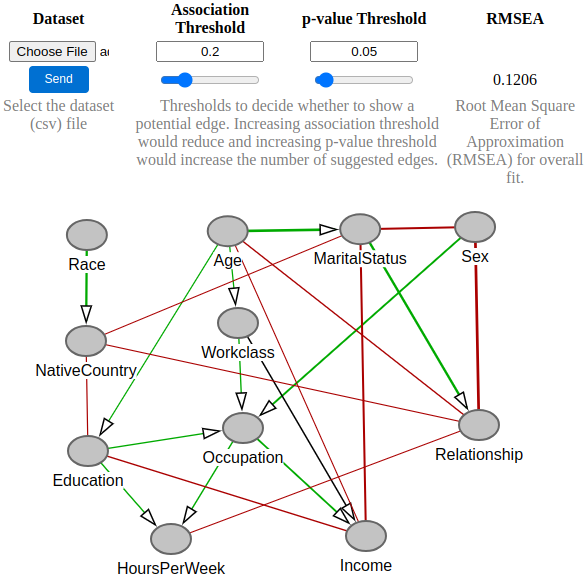
\includegraphics[scale=0.4]{../code/plots/web_tool_full_new.png}
	\caption{A screenshot of the web tool for constructing the model. Users
		can upload their dataset after which the tool creates an empty
		graph and shows all pair of variables which are associated in
		the model using undirected red edges with the strength of
		association represented using edge width. Users can then
		iteratively add edges to the model (shown in green) while
		deciding the edge orientation based on domain knowledge.
		Unnecessary edges are shown in black.}
	\label{fig:web}
\end{figure}

To enable users to apply this method to their own datasets, we developed an
interactive web-based tool (shown in Fig.~\ref{fig:web}) for constructing
models. Users begin by uploading their dataset, which initializes an empty DAG
with nodes corresponding to the dataset\'s variables. They can then specify a
p-value threshold and a measure of association threshold. We use the measure of 
conditional association shown in Appendix~\ref{sec:mixed_association}. 

Using the specified thresholds, the tool visually highlights unexplained
correlations by displaying red edges between variables where correlation exists
in the data but the current DAG is not able to explain. The thickness of these
edges represents the strength of the correlation, helping users prioritize
which edges to add. Similarly, if an edge in the graph is detected to be
unnecessary, it is highlighted in black. Based on this information, users can
select to remove unnecessary edge or select a potential edge to add and specify
the orientation of the edge. The tool computes Shipley’s C \citep{Shipley2000}
value at each change to determine the overall fit of the model to the data.
Once satisfied with the constructed DAG, users can export the model for further
analysis.


\section{Conclusions}

Points:
\begin{itemize}
	\item As researchers prefer to build models by hand, we present a tool
		to assist them in construction using CI testing.
	\item In practice as many edges are possible for any given DAG, we provide
		a ranking method to find the best edge addition.
	\item Compared to other expert knowledge specification methods, users
		don't need to guess what information then need to provide as
		exact questions are asked. Also enables us to ask an LLM for
		it.
\end{itemize}

Future work:
\begin{itemize}
	\item Add latent variables; extend to ADMGs.
	\item Can potentially be combined with pairwise orientation methods.
	\item Improvements in the web-interface.
\end{itemize}

\bibliography{references}

\newpage

\onecolumn
\title{Expert-In-The-Loop Causal Discovery: Iterative Model Refinement Using Expert Knowledge \\ (Supplementary Material)}
\maketitle
\appendix

\section{Prompts Used for LLM}
\label{section:llms}

\begin{figure}[ht!]
	\centering
	\begin{verbatim}
You are an expert in Social Science. Following are the descriptions of two variables:

<A>: {description of variable A}
<B>: {description of variable B}

Which of the following two options is the most likely causal direction between these 
variables:

1. <A> causes <B>
2. <B> causes <A>

Return a single letter answer between the choices above; Do not provide any reasoning 
in the answer; Do not add any text formatting to the answer.
	\end{verbatim}
	\caption{Prompt used for the LLM. Here the variable descriptions are replaced with description provided in Fig.~\ref{fig:var_description}}
	\label{fig:prompt}
\end{figure}

\begin{figure}[ht!]
	\begin{verbatim}
          Age: The age of a person
    Workclass: The workplace where the person is employed such as Private industry, 
     	       or self employed
    Education: The highest level of education the person has finished.
MaritalStatus: The marital status of the person
   Occupation: The kind of job the person does. For example, sales, craft repair, 
   		clerical.
 Relationship: The relationship status of the person.
         Race: The ethnicity of the person.
          Sex: The sex or gender of the person.
 HoursPerWeek: The number of hours per week the person works.
NativeCountry: The native country of the person.
       Income: The income i.e. amount of money the person makes.
	\end{verbatim}
	\caption{Variable descriptions used for prompting the LLM}
	\label{fig:var_description}
\end{figure}

\section{A Generalized Measure of Conditional Association}
\label{sec:mixed_association}

In the previous section, we discussed how different types of variables require
different measures of conditional association. However, there is no unified
measure that handles mixed data. In this section, we introduce a measure of conditional
association for mixed data by extending the concept of partial correlation
coefficient (commonly used for continuous variables) to mixed data. Similar to
partial correlation coefficient, our method integrates a mixed data
residualization method \citep{Ankan2023} with Pillai's Trace
\citep{Pillai1955}, a multivariate measure of association based on canonical
correlations.
 
Given a dataset $ D = (x, y, \bm{z}) $ on variables $ X $, $ Y $, and $ \bm{Z}
$, our goal is to estimate the conditional association $ \phi_{X, Y; \bm{Z}} $. 
In the first step, we compute the residuals $ R_X $ and $ R_Y $ for variables
$ X $ and $ Y $ respectively. Depending on the type of variable the residual
is computed as follows:

\begin{enumerate}
	\item \textbf{Continuous:} We train a model, $ E_X: x \sim
		\bm{z} $. The residuals are then computed by taking the difference
		between the true and the predicted values using $ E_X $. 
		$$ R_{x_i} = x_i - E_X(\bm{z}_i) $$
	\item \textbf{Ordinal:} We start by training a probability estimator, $
		p_X: x \sim \bm{z} $, and then use the estimated probabilities, 
		$ \hat{p}_X(x) $ to compute the residuals:
		$$ R_{x_i} = \hat{p}_X(X < x_i) - \hat{p}_X(X > x_i) $$
	\item \textbf{Categorical:} We again start by training a probability
		estimator $ p_X: x \sim \bm{z} $, and obtain probability
		estimates $ \hat{p}_X: p_X(\bm{z}) $. Next, we dummy encode the
		categorical variable, resulting in a binary vector and then
		compute the residuals as follows: 
		$$ R_{x_i} = x_i - \hat{p}_X(\bm{z}_i) $$
\end{enumerate}

We have the option here to choose the estimators based on the characteristics
such as distribution, type of relationship, and so on of our dataset.
Non-parametric ensemble estimators such as Random Forest and XGBoost are robust 
for diverse data types and complex relationships. For linear relationships,
simpler models such as linear regression and its variants may suffice.

We repeat the above residualization step for both the variables $ X $ and $ Y $
obtaining residual matrices $ R_x $ and $ R_y $. The type of variable determines
the shape of these matrices. If the variable is continuous or ordinal, the 
residual matrix is of shape $ (n \times 1 ) $ and if the variable is categorical,
we get a residual matrix of shape $ (x \times (k - 1)) $, where $ k $ is the number
of categories of the variable.

The second step is to quantify the association between these residual matrices.
For this purpose we use canonical correlations \citep{Hotelling1936} that have been widely used to
measure the association between sets of random variables.

\begin{definition}
	Given two sets of random variables $ \bm{U} = (U_1, U_2, \cdots, U_p) $
	and $ \bm{V} = (V_1, V_2, \cdots, V_q) $, canonical correlation between
	them, $\rho_{\bm{U}, \bm{V}} $ is defined as:
		
	\begin{equation}
		% \nu_{\bm{U}, \bm{V}}= \max_{a, b} \mathrm{corr}(a^T \bm{U}, b^T \bm{V})
		\rho_{\bm{U}, \bm{V}} = \max_{a, b} \frac{a^T \Sigma_{\bm{UV}} b}{\sqrt{a^T \Sigma_{\bm{UU}} a \cdot b^T \Sigma_{\bm{VV}} b}}
	\end{equation}

	where $ a $ and $ b $ are vectors of coefficients that maximize the correlations
	between the linear combinations of $ a^T \bm{U} $ and $ b^T \bm{V} $.
\end{definition}

Canonical correlations generalize the concept of correlation coefficients to
multi-dimensional variables. It finds orthogonal linear transformations $ a $
and $ b $ that maximized the correlation between the transformed variables $
a^T \bm{U} $ and $ b^T \bm{V} $. This yields a vector of correlation
coefficient values of size $ \min(p, q) $, representing the correlation
coefficient of each pair of transformed variables. Notably, Pearson's
correlation coefficient is a special case of canonical correlations when $ p =
q = 1 $.

Several measures of association have been derived from canonical correlations, such as:
\begin{itemize}
	\item Wilks' Lambda: $\Lambda = \prod_{i}^{\min(p, q)} (1 - \rho_i^2) $
	\item Roy's Largest Root: $ \theta = \max_i(\rho_i^2) $
	\item Pillai's Trace: $ \tau = \sum_{i=1}^{\min(p, q)} \rho_i^2 $
\end{itemize}

We use a normalized version of Pillai's Trace for our purpose, given as:

\begin{equation}
	\tau_{X, Y; \bm{Z}} = \frac{1}{\min(\rvert R_x \rvert, \rvert R_y \rvert)}
	\sum_{i=1}^{\min(\rvert R_x \rvert, \rvert R_y \rvert)} (\rho_{R_x, R_y})_i^2
\end{equation}


We use Pillai's Trace because: 1) It uses all the canonical correlation values,
capturing the full extent of association, 2) Its interpretation is similar to
Pearson's correlation coefficient, i.e., $ 0 $ signifies no association and $ 1
$ signifies perfect linear relationship. We use a normalized version because
when comparing between pair of variables with different number of categories.
Our proposed measure has several desirable properties that make it well-suited
for our application:

\begin{enumerate}
	\item \textbf{Bounded: } The measure is bounded between $ 0 $ (no
		association) to $ 1 $ (perfect linear association), simplifying
		interpretation.
	% \item \textbf{Independent of Sample Size: } 
	\item \textbf{Invariant to the Dummy Encoding: } For categorical
		variables, residuals are computed using dummy encoding. Since
		canonical correlations identifies linear combinations across
		columns, this measure is invariant to the specific dummy
		encoding scheme used.
	\item \textbf{Equivalent to Partial Correlation for Continuous Variables: }
		When both $ X $ and $ Y $ are continuous variables, our measure
		is equivalent to the absolute value of partial correlation coefficient.
	\item \textbf{Equivalent to polychoric and polyserial correlation for
			ordinal and continuous variables: }
		Under the assumption that the ordinal variable is generated by
		discretizing an underlying gaussian continuous variable, this
		effect size is equivalent to polychoric and polyserial
		correlation. As both of them recover the Pearson correlation
		coefficient.
		\todo[inline]{Verify if this is correct}
	\item \textbf{Related to Cram\'er's V: } 
\end{enumerate}

In essence, our measure of conditional association extends existing metrics to mixed data, providing 
a unified measure that is interpretable.

\end{document}
